% !TeX spellcheck = de_DE
\section{Strategien zur Datenmigration}
\label{chapter:strategien}
%TODO Tobias

Als Kernelement der Datenmigration stehen unterschiedliche Strategien zur Verf"ugung. Unterschiedliche Ans"atze fokussieren dabei je die Ebenen Datenquellen und Anwendung. Einzelne Strategien bieten Vor- und Nachteile. Sie sind von unterschiedlichen Gruppen innerhalb eines Unternehmens oder Migrationsprojektes vorzunehmen.

\subsection{Generelles Vorgehen}

Unabh"angig von der gew"ahlten Strategie setzt die Durchf"uhrung einer Datenmigration drei grunds"atzliche T"atigkeiten voraus \citep{henrard-2002}. Diese dienen als Ger"ust der Umsetzung einer Migration. 

\begin{itemize}
	\item \textbf{Konvertierung der Datenhaltungs-Schemata} \\
	Erkennen und Analysieren von vorhandenen Schemata und Datenformaten. Auf Basis der existierenden Datenformate wird unter Umst"anden eine Neukonzeptionierung der Formate vorgenommen. Anpassungen m"ussen die Erhaltung der bereits vorhandenen Datenber"ucksichtigen und neue Schemata auf Basis der Ziel-Technologie etablieren.
	\item \textbf{Konvertierung der Daten} \\
	Ist die Konvertierung der Schemata erfolgt, m"ussen die Daten selbst in das neue Format gebracht werden. Eine Automatisierung durch Umkopieren der Daten vom alten in das neu Format verk"orpert die Konvertierung.
	\item \textbf{Anpassung der Anwendung} \\
	Sind Daten und Schemata konvertiert, m"ussen angrenzende Softwaresystem angepasst werden. Anwendungen, welche alte Datenformate und -technologien nutzen, m"ussen auf die Nutzung der neuen Formate hin angepasst werden.
\end{itemize}

Migrationen erfolgen prinzipiell auf zwei Ebenen \citep{henrard-2002}. Datenbanken und -quellen bilden die grundlegende Ebene. Schemata der Datenhaltung m"ussen angepasst und konvertiert werden. Vorliegende Daten werden analysiert. Die zugrundeliegenden Strukturen werden "uberarbeitet oder angepasst. Sie werden in einigen F"allen auf andere Technologien "ubertragen. Sind Schemata angepasst, m"ussen vorhandene Daten "ubertragen und, sofern erforderlich, in neue Formate konvertiert werden.
\lb
In Folge der Migration der Daten selbst m"ussen umliegende Softwaresysteme mit Zugriff auf diese Daten ihre Nutzung der Datenquellen anpassen. Da unter Umst"anden Schnittstellen und Datenformate ver"andert werden, muss die spezifische Nutzung dieser der Evolution auf Datenbankebene angepasst werden. 

% == 
\subsection{Datenbankebene}

Auf Ebene der Daten erfolgt sinnvollerweise eine Anpassung von zugrundeliegenden Technologien, Datenbankschemata oder Datenformaten. Gr"unde f"ur eine Migration auf dieser Ebene finden sich auf Ebene der Hintergr"unde des zugrundeliegenden Reengineerings. Sie reichen von einem Wechsel auf zukunftssichere Technologien oder einer Anpassung von Gesch"aftsprozessen. Unterschiedliche Ans"atze beg"unstigen oder hemmen dabei das Erreichen eben dieser Ziele. 

% ===
\subsubsection{Physisch}

Die Migration von Daten auf physischer Ebene schlie"st die Konvertierung von Datenformaten und -schemate auf rein struktureller Ebene ein. Daten werden dabei ohne Betrachtung der semantischen Zusammenh"ange auf neue Formate oder Technologien "ubertragen. Beispiel ist etwa die Abbildung relationaler Datenmodelle auf Objekt-orientierte Schemata \citep{alhajj-2001}, \citep{behm-1997}. Dabei werden Daten und ihre Modellierung in ein neues Schema "ubertragen, fachlich dennoch nicht ver"andert.
\lb
Grunds"atzlich muss zun"achst das vorhandene Format der Daten analysiert werden. Aus den gewonnenen Erkenntnissen kann die "Ubersetzung auf neue Schemata und Strukturen erfolgen. Sind, etwa beim Wechsel eines Datenbankformates in ein anderes keine "aquivalenten Konstrukte vorhanden, m"ussen Strukturen, welche diesen am "ahnlichsten sind, gew"ahlt werden. 
\lb
Sind Datenformate und Schemata konvertiert und angepasst m"ussen vorhandene Daten in die neue Umgebung eingef"ugt werden. In diesem Schritt ist das kopieren der Daten aus dem urspr"unglichen Format in die neue Umgebung vorgesehen. Unter Umst"anden m"ussen Datens"atze konvertiert werden. Skripte und Tools zur Unterst"utzung begleiten diesen Prozess \citep{henrard-2002}.
\lb
Abbildung \ref{pic:conversion_physical} zeigt am Beispiel von Datenbanken eine physische Konvertierung. Das vorliegende DDL\footnote{\textit{Data Definition Language} - Sprache zur Beschreibung von Datenformaten}-Schema des Quell-DMS\footnote{\textit{Data Management System} - Datenbank-Verwaltungs-System} wird analysiert. Die entstandene Abbildung des SPS (\textit{Source Physical Schema}) wird in ein TPS (\textit{Target Physical Schema}) konvertiert. Diese "Ubersetzung des Schemas muss letztendlich innerhalb des Ziel-DMS kodiert werden \citep{henrard-2002}.

\begin{figure}[h!]
	\centering
	\caption{Physische Konvertierung}
	\label{pic:conversion_physical}
	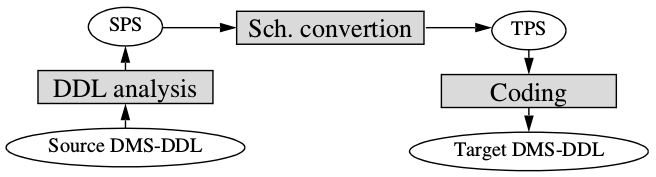
\includegraphics[width=0.9\textwidth]{../images/strategies_fig_02a.png} \\
	\tiny Quelle: \citep{henrard-2002}, Abbildung 2
\end{figure}

Durchf"uhrung auf physischer Ebene sind meist elementare Konvertierungen und m"ussen nicht zwangsweise von Analysten oder fachlich geschultem Personal vorgenommen werden. Die rein physische Konvertierung kann automatisiert durchgef"uhrt werden \citep{abiteboul-1999}.
\lb
Nachteil der physischen Konvertierung ist ein fehlender Mehrwert der entstandenen Daten \citep{henrard-2002}. Vorhandene Schemata werden soweit wie m"oglich auf andere Technologien "ubertragen. Eine fachliche und konzeptuelle Analyse der Daten bleibt aus. In diesem Fall stellt die Migration der Daten lediglich ein Umkopieren in ein neues Datenformat dar.
\lb
Die physische Migration eignet sich vor allem bei einem Wechsel der technischen Umgebung der Daten, etwa einem Wechsel der Version des verwendeten DMS oder einem Wechsel des Herstellers. %TODO Finish

% ===
\subsubsection{Konzeptuell}

Anders als auf physischer Ebene werden Daten auf konzeptueller Ebene auch semantisch betrachtet. Schemata und Datenformate werden evaluiert und neu konzeptioniert. Aus der fachlichen Betrachtung der Daten ergeben sich unter Umst"anden umfangreiche "Anderungen an den Schnittstellen der System. Fachliche Konvertierung erfordern ein Umdenken. Dieses kann die Qualit"at der migrierten Daten verbessern.
\lb
Die konzeptuelle Migration der Daten f"uhrt auf vorhandenen Schemata und Datenformaten eine semantische Analyse durch. Anhand der aus dieser gewonnenen Informationen wird eine Neukonzeptionierung der Modellierung vorgenommen. Abbildung \ref{pic:conversion_conceptual} zeigt das Vorgehen w"ahrend der konzeptuellen Migration. Das Quell-DMS Schema wird mithilfe eines Database Reengineering (BDRE) analysiert \citep{henrard-2002}. Ziel dieses Vorganges ist die Bereinigung (engl.: \textit{Cleansing}) vorhandener Daten \citep{rahm-2010} \citep{hernandez-1998}. Auf Basis einer neuen Konzeptualisierung des der Schemata wird die Konvertierung "ahnlich zur physischen Migration vorgenommen. Neue Formate werden in das Ziel-Format "ubertragen und kodiert. Die Konvertierung und Migration der eigentlichen Daten in die neue Umgebung erfolgt ebenfalls mithilfe von Konvertierungen. Diese ist, im Gegensatz zur physischen Konvertierung, umfangreicher. Neue Abbildungen und Modellierungen m"ussen aus vorhandenen Daten abgeleitet werden. In diesem Zusammenhang spielt auch das Reengineering der Anforderungen an die zugrundeliegenden Daten eine Rolle \citep{aiken-1994}.

\begin{figure}[h!]
	\centering
	\caption{Konzeptuelle Konvertierung}
	\label{pic:conversion_conceptual}
	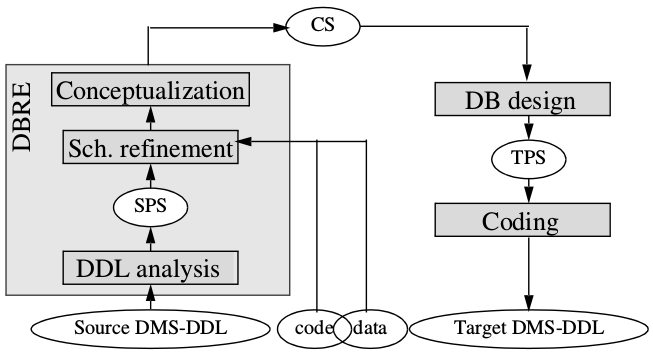
\includegraphics[width=0.9\textwidth]{../images/strategies_fig_02b.png} \\
	\tiny Quelle: \citep{henrard-2002}, Abbildung 2
\end{figure}

Auf konzeptueller Ebene spielt die fachliche Betrachtung vorhandener Daten eine wichtige Rolle. Das Verfahren ist nicht zwangsweise trivial. Analysen und konzeptuelle Konvertierung ben"otigen ein gewisses Verst"andnis der Semantik von Daten.
\lb
Eine konzeptuelle Migration von Daten sorgt vor allem f"ur ein saubere Portierung vorhandener Daten. Schemata werden semantisch korrekt an neue Umgebungen und Formate angepasst. Eine potentielle S"auberung der Daten verringert unter Umst"anden Redundanzen oder nicht ben"otigte Datens"atze oder -formate.
\lb
Der f"ur eine konzeptuelle Migration notwendige Aufwand ist vergleichsweise hoch. Ben"otigte Spezialisten und erforderliches fachliches Verst"andnis von Daten und Umgebung sorgen eventuell f"ur hohe Kosten.
\lb
Fazit %TODO

% ==
\subsection{Anwendungsebene} %TODO Needs more citations :P

Sind Datenformate und Daten selbst konvertiert und migriert, m"ussen umgebende Softwaresysteme angepasst werden. Ver"anderte Datenformate beziehungsweise Technologien setzen oft einen ver"anderten Zugriff auf diese Daten voraus. Um den Aufwand f"ur "Anderung innerhalb der nutzenden Anwendungen m"oglichst zu reduzieren, existieren drei Strategien der Anpassung von Anwendungen. Die zeichnen sich durch unterschiedliche Ebenen der Anpassung aus. Je nach Tiefe der Anpassung liegen ihnen unterschiedliche Ans"atze zugrunde. 

% ===
\subsubsection{Wrapper}

Um den Aufwand f"ur "Anderungen innerhalb von Softwaresystemen gering zu halten, bietet sich die Implementation eines Wrappers oder Adapters an. Dieser stellt eine Schnittstelle zwischen dem urspr"unglichen, unver"anderten Anwendungssystem und der neu strukturierten Datenquelle dar. Der Wrapper wird dabei als zus"atzliche Schicht zwischen beiden Komponenten eingef"ugt. Er nimmt Aufrufe der urspr"unglichen Anwendung entgegen, "ubersetzt sie in Anfragen an die neue Datenquelle und konvertiert die Ergebnisse der Anfrage f"ur das urspr"ungliche System. Er fungiert als Vermittler zwischen beiden Systemen und erspart so den Aufwand umfangreicher "Anderungen f"ur Abfragen im Anwendungssystem.
\lb
Abbildung \ref{pic:application_wrapper} zeigt das Schema zur Nutzung eines Wrappers. Die Abstraktion erfolgt dabei auf Basis von Prozeduren zum Aufruf der neuen Datenquelle durch den Wrapper. Vor der Einbindung des Wrappers m"ussen diese in die Legacy-Anwendung eingef"ugt werden. Nur so kann der sp"atere Aufruf des Wrappers anstatt der urspr"unglichen Datenquelle erfolgen \cite{henrard-2008}. 

\begin{figure}[h!]
	\centering
	\caption{Einsatz eines Wrappers auf Anwendungsebene}
	\label{pic:application_wrapper}
	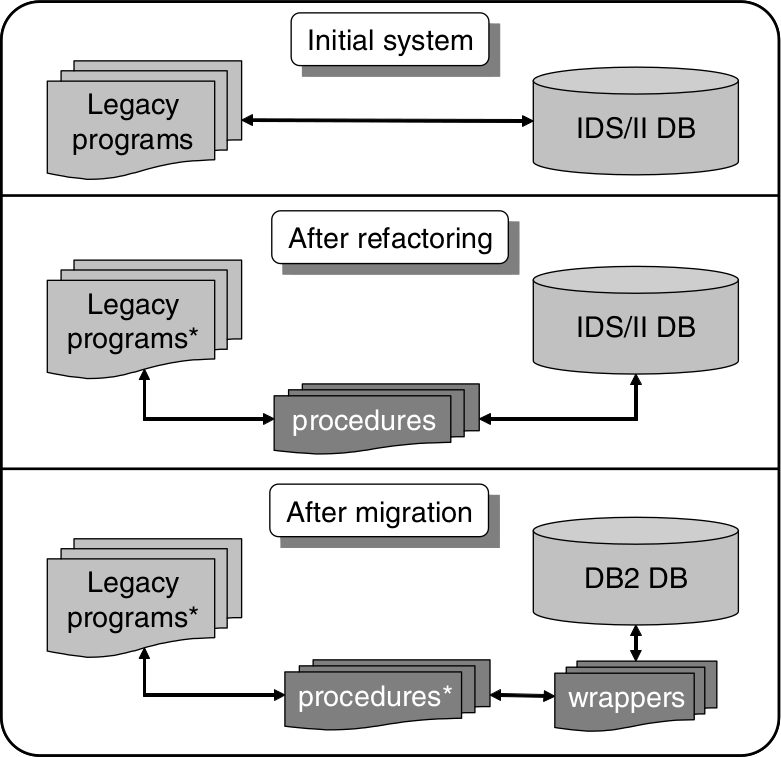
\includegraphics[width=0.5\textwidth]{../images/large_scale_fig_01.png} \\
	\tiny Quelle: \citep{henrard-2008}, Abbildung 1
\end{figure}

Ein fiktives Legacy-System dient der Illustration. Zu seinen Aufgaben geh"ort der Zugriff auf Kundendaten. Diese werden im Legacy-System mit naiven Mitteln zur Datenhaltung verwaltet \citep{henrard-2002}. Beispiel \ref{code:wrapperbefore} zeigt den urspr"unglichen Aufruf der Datenquelle. Das nachfolgende Beispiel \ref{code:wrapperafter} illustriert den neuen Zugriff auf den Wrapper. Die Anpassung an dieser Schnittstelle ist gering \citep{henrard-2002}\footnote{Die Quellcode-Beispiele auf den folgenden Seiten sind aus \citep{henrard-2002} entnommen und dienen nur der Illustration}.

\lstinputlisting[label=code:wrapperbefore,caption=Beispiel Legacy-Programm mit Aufruf der urspr"unglichen Datenquelle]{../src/wrapper_legacy.cbl}

\lstinputlisting[label=code:wrapperafter,caption=Beispiel Legacy-Programm mit Aufruf der urspr"unglichen Datenquelle]{../src/wrapper_new.cbl}

Deutlicher Vorteil in der Verwendung eines Wrappers ist die notwendige geringe "Anderung des Anwendungssystems. Der Einsatz eines Wrappers gef"ahrdet die Integrit"at des nutzenden Softwaresystems nur sehr gering. Das Risiko wird dabei minimiert.
\lb
Durch Implementation eines Wrappers entsteht zus"atzlicher Aufwand f"ur die Implementation und Integration des Wrappers in die bestehende Systemlandschaft.
Nachteile
\lb
Erfolgt der Zugriff auf eine Datenquelle an vielen Stellen im Quellcode der Legacy-Anwendung, ist die Einf"uhrung eines Wrappers mit vergleichsweise wenig Aufwand verbunden. Anders als die Anpassung von Aufrufe oder der Ver"anderung der Programmlogik, reduziert sich die Einf"uhrung eines Wrappers auf das Austauschen der Aufrufe der Datenquelle. Verarbeitung und Nutzung der Datenquelle werden vom Wrapper wie in der urspr"unglichen Quelle bereitgestellt. Die relativ simple Anpassungen beim Einsatz eines Wrappers und ein sehr geringer Aufwand f"ur die Anpassung im Legacy-System selbst sind die Vorteil bei Nutzung eines Wrappers. Entgegen dem geringen Aufwand im System selbst, erfordert die Implementation eines Wrappers entsprechendes technische Verst"andnis sowohl der neuen als auch der alten Datenquelle. Dies garantiert die korrekte Nutzung der Daten durch die Legacy-Anwendung. Durch den bestehenden Umfang der Nutzung durch das Legacy-System k"onnen technische M"oglichkeiten der neuen Datenquelle unter Umst"anden nicht genutzt werden.

% ===
\subsubsection{Statements}

Eine detailliertere Anpassung der Anwendungssysteme stellt das Anpassen der Aufrufe der Datenquelle dar. Der Zugriff auf Daten erfolgt durch entsprechende Anweisungen im Quellcode einer Anwendung. Die Anpassung entsprechender Statements im Quellcode nimmt dabei die Anpassung des Anwendungssystems vor. Anpassungen in entsprechenden Statements sind der Kern dieser Strategie. Es wird lediglich der tats"achliche Zugriff auf die Datenquelle ver"andert, nicht jedoch sein Struktur. Sind umfassende "Anderungen im Bezug auf die eingesetzte Technologie durchgef"uhrt worden, reicht eine blo"se Anpassung der Statements unter Umst"anden nicht aus.
\lb
Beispiel \ref{code:statementbefore} zeigt den Aufruf der Datenquelle vor Anpassung der Statements. Die Anpassung in Beispiel \ref{code:statementeafter} verdeutlicht die Anpassung. Wo zuvor der Zugriff mit Sprachmitteln des Legacy-Systems erfolgte, sind Statements nach der Anpassung auf die Nutzung von SQL ausgelegt. Die entsprechenden Anpassungen sind umfangreicher als die Nutzung eines Wrappers.

\lstinputlisting[label=code:statementbefore,caption=Aufruf der Datenquelle vor Anpassung der Statements]{../src/statementrewrite_cobol.cbl}

\lstinputlisting[label=code:statementeafter,caption=Aufruf der neuen Datenquelle: Zugriff via SQL]{../src/statementrewrite_sql.cbl}

Vorteil der Anpassung von Statements ist eine technisch saubere L"osung. Anpassungen an den Abfragen, etwa "Anderungen an SQL-Statements, sind eher simpel in der Durchf"uhrung. Die "Anderung der Statements erfordert nicht zwangsweise ein tiefgreifendes Verst"andnis des Anwendungssystems. 
\lb
Anpassungen an Statements reagieren auf eine Ver"anderte Schnittstelle der Datenquelle. Gr"o"sere strukturelle oder konzeptionelle "Anderungen k"onnen jedoch nicht ber"ucksichtigt werden.
\lb
Das Anpassen von Statements im Anwendungssystem ist sinnvoll, wenn an nur wenigen Stellen im Quellcode Anpassungen vorgenommen werden. Ist etwa der Zugriff auf die Datenquelle gekapselt, ist die Anpassung nur in geringem Umfang durchzuf"uhren. Im Gegensatz zum Einsatz eines Wrappers an der Schnittstelle, ist die "Anderung von Statements eine integrierte L"osung und greift in das Anwendungssystem ein. Um die Anpassung korrekt durchf"uhren zu k"onnen, ist ein grundlegendes Verst"andnis der betreffenden Anwendung notwendig.

% ===
\subsubsection{Logik}

Um alle M"oglichkeiten neuer Datenquellen und -technologien nutzen zu k"onnen, muss unter Umst"anden die Logik des zugreifenden Anwendungssystemes ver"andert werden. Dabei werden Datenstrukturen, Algorithmen und Zugriff innerhalb der Software massiv ver"andert, um auf die neue Umgebung zu reagieren \citep{henrard-2002}.
\lb
F"ur eine Anpassung der Logik ist es erforderlich, entsprechende Passagen innerhalb der Anwendungssoftware an die neue Datenquelle anzupassen. Beispiel \ref{code:logicbefore} zeigt den urspr"unglichen Zugriff des Legacy-Systems. Die angepasst Logik ist in Beispiel \ref{code:logicafter} einzusehen. Als Unterschied zur reinen Anpassung der Statements sind die Auswirkungen auf andere Programmteile meist gr"o"ser \citep{henrard-2002}.

\lstinputlisting[label=code:logicbefore,caption=Ursp"ungliche Logik f"ur den Zugriff auf die Datenquelle]{../src/logic_before.cbl}

\lstinputlisting[label=code:logicafter,caption=Angepasste Zugriffslogik f"ur Datenquelle in SQL]{../src/logic_after.cbl}

Die Anpassung der Logik und damit potentiell die Nutzung aller M"oglichkeiten der neuen Datenquellen beziehungsweise Schnittstelle erh"oht den Nutzen der Anwendungssoftware. Kann das Softwaresystem von den neuen M"oglichkeiten Gebrauch machen, erh"oht dies m"oglicherweise den Gesch"aftswert der Komponente. 
\lb
Hinter der Anpassung der Logik eines Anwendungssystemes verbirgt sich immer ein gewisses Risiko. Je umfangreicher die "Anderungen ausfallen, desto h"oher ist das Risiko. Gerade funktionale "Anderungen, wie der Zugriff und die Arbeit mit Datenquellen, kann ein hohes Risiko beim Reengineering von Legacy-Systemen mit sich bringen.
\lb
Neben dem Einsatz eines Wrappers und der Anpassung von Statements bildet die Anpassung der Logik die umfangreichste Strategie auf Anwendungsebene. Die Umsetzung erfordert umfassendes Verst"andnis der fachlichen Logik des betreffenden Softwaresystems. Wie die bereits genannten Ans"atze stellt sich auch die Anpassung der Logik durch Vor- und Nachteile dar. Unterschiedliche Strategien und Ans"atze k"onnen die Migration auf unterschiedlichen Ebenen unterst"utzen. Welche Strategie einzusetzen ist, h"angt stark vom Kontext, dem bestehenden Legacy-System und dem technischen und fachlichen Wissen der Beteiligten eines Migrationsprojektes ab.